%lensed_waveguide_extension
Besides the previous discussion about the lensed waveguide, there are more operations we can resort to. From \cite{integrated_coupling_between_LD_SMF} more ideas can be found to promote the coupling efficiency between TLF and lensed waveguide. The author has presented a tapered core fiber like Fig.\ref{fig:tapered_core_fiber}, which is capable to confine more beam rays. In this configuration there is a small distance $h_{1}$ between the lens end $H_{1}$ and core interface $H_{2}$, because the lens end is not the exact minimum spot location for a lensed waveguide. Thus it is possible to gain a higher coupling efficiency, if the distance between the lens and the core is expanded properly and this part of waveguides can be named as 'neck' (see Fig. \ref{fig:lensed_waveguide_neck}).\\ 

\begin{figure}[!ht]
\centering
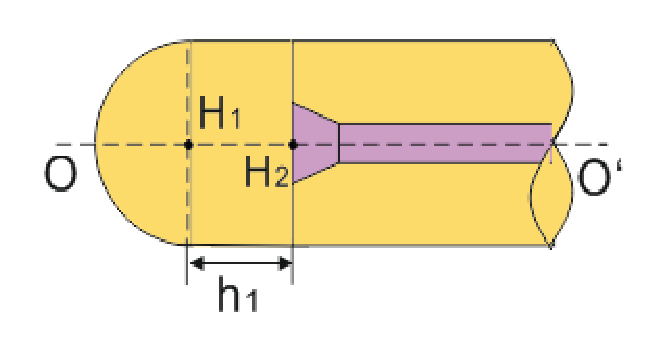
\includegraphics[width=0.6\textwidth]{bilder/tapered_core_fiber}
\caption {Schema of tapered core fiber\cite{integrated_coupling_between_LD_SMF}.}
\label{fig:tapered_core_fiber}
\end{figure}
\begin{figure}[!ht]
\centering
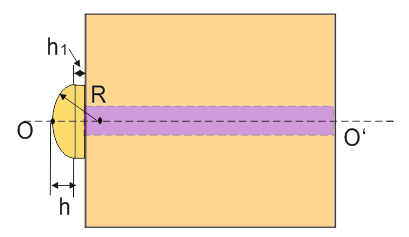
\includegraphics[width=0.7\textwidth]{bilder/lensed_waveguide_neck}
\caption {Schema of a lensed buried waveguide with a 'neck'.}
\label{fig:lensed_waveguide_neck}
\end{figure}
For a proper 'neck' length $h_{1}$ higher coupling efficiency should be achieved. Through brief simulations in Fig. \ref{fig:s21_neck}, we can conclude that neck length does affect the coupling efficiency. Because this setup has 3 variables (lense hight, lens radius and neck length), more research can be done for the optimal arrangement.\\

\begin{figure}[!ht]
\centering
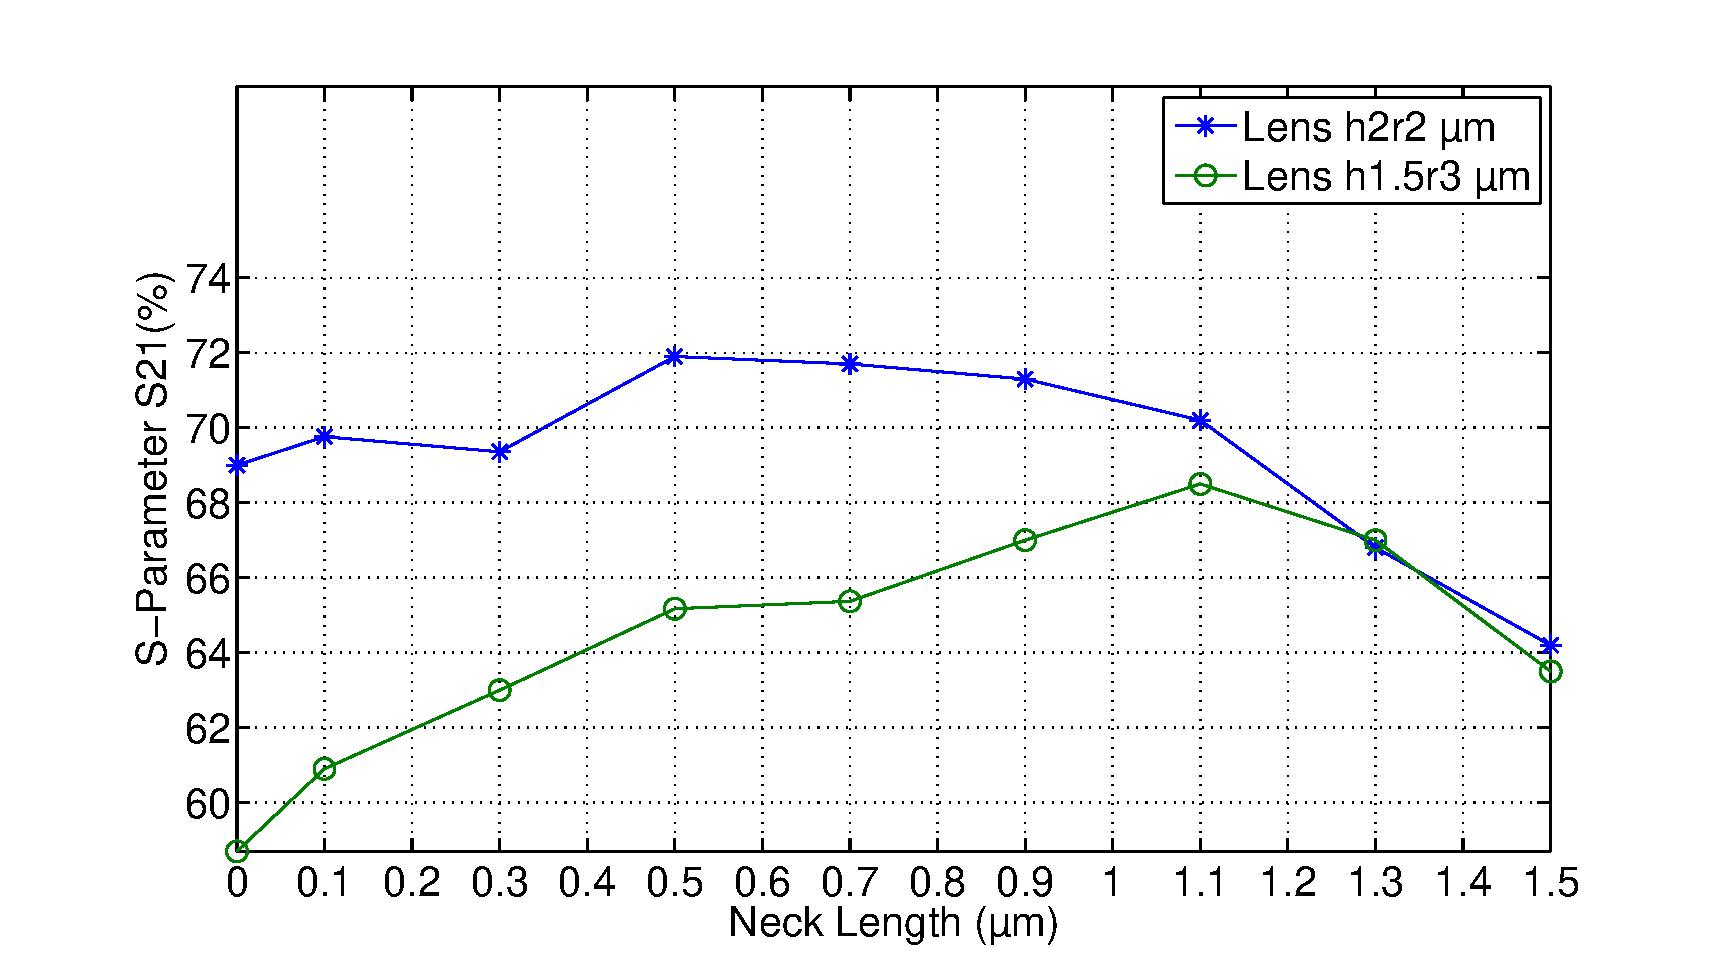
\includegraphics[width=0.9\textwidth]{bilder/s21_neck}
\caption {Schema of coupling efficiency due to 'neck length'. Curve 'Lens h2r2' presents the configuration of lens height=2$\mu$m, radius=2$\mu$m. Curve 'Lens h2r2' presents the configuration of lens height=1.5$\mu$m, radius=3$\mu$m.}
\label{fig:s21_neck}
\end{figure}
